La fase di \textit{Interest Dissemination} è una procedura molto importante per il corretto funzionamento di GreenWUP. In particolare questa fase viene realizzata attraverso un protocollo di \textit{flooding} chiamato FloodWUP, descritto in \cite{greenWup}. \\

L'obbiettivo principale di questo protocollo è far si che ogni nodo della rete riesca a impostare la propria distanza dal sink (espressa in numeri di hop, ovviamente).\\
Da qui in avanti si farà riferimento a questo valore mediante il termine \textit{hopCount}.\\ 

La procedura ha inizio con l'invio di una pacchetto chiamato \textit{disseminationPacket} (per semplicità DP) da parte del sink. Questo pacchetto conterrà il valore che i vari nodi useranno come proprio hopCount. In particolare questo valore vale 0 solo per il sink, mentre ogni nodo che riceve il pacchetto memorizza il proprio valore come \( valore\_pacchetto + 1 \). \\

Una particolarità molto importante di questo protocollo è che il traffico generato, seppur l'invio segua un process di broadcast, non genera \textit{broadcast storm}. Ciò è ovviamente possibile grazie all'uso dei messaggi di wake-up e grazie al fatto che ogni nodo usa un pool condiviso di indirizzi di wake-up \(w_1, w_2....w_n\).\\
Inizialmente i vari nodi usano l'indirizzo \(w_1\) per cui il sink, così come gli altri nodi, durante l'invio del primo DP sveglierà i propri vicini usando l'indirizzo \(w_1\). Ogni nodo, dopo aver ricevuto il DP, procede a cambiare indirizzo di wake-up da \(w_1\) a \(w_2\) e a ridistribuire il DP corrente ai suoi vicini usando però l'indirizzo con cui sono stati svegliati (nel caso del primo pacchetto DP \(w_1\)).\\

Con l'invio del secondo DP, invece, i vari nodi useranno allo stesso modo \(w_2\), così come per il terzo DP useranno \(w_3\) e così via. Questo permette di evitare il \textit{broadcast storm} in quanto i nodi che hanno già ricevuto un pacchetto DP, avendo aggiornato la sequenza di wake-up, non riceveranno duplicati di questo.

\begin{listing}[h]
    \caption{Procedura usata dal Sink per creare un nuovo DisseminationPacket}
    \label{code:createDP}
    \begin{minted}[mathescape, linenos, numbersep=10pt, gobble=0, fontsize=\small, frame=lines, framesep=2mm]{cpp}

GreenWupPacket* macFrame;
macFrame = new GreenWupInterest("GreenWupInterest", MAC_LAYER_PACKET);

// Informazioni per DisseminationPacket
macFrame->setWurAddress(wurDisseminationAddresses[fromNetAddressIndex]);
macFrame->setType( PKT_GREEN_WUP_INTEREST );
macFrame->setHc(level);
int size = wurDisseminationAddresses.size();
fromNetAddressIndex = ( fromNetAddressIndex + 1 ) % ( size );

// Informazioni Generiche
encapsulatePacket(macFrame, pkt);
macFrame->setDestination(destination);
macFrame->setNetAddress(self);
macFrame->setNetSN(netSN++);
macFrame->setSource(SELF_MAC_ADDRESS);

    \end{minted}
\end{listing} \\

Come mostrato nel \textbf{Codice \ref{code:createDP}}, il nodo sink imposta alcuni parametri come \textit{sequenza di wake-up}, il \textit{tipo del pacchetto} (usato dai vicini che ricevono il pacchetto in modo da gestirlo nel corretto modo) e ovviamente l' \textit{hopCount}. Fatto ciò aggiorna il prossimo indirizzo di wake-up da usare (\textbf{linea 9, Codice \ref{code:createDP}}) e invia il pacchetto in broadcast. \\

Ciò che invece mostra il \textbf{Codice \ref{code:forwardDP}} è il modo in cui i vari nodi gestiscono il \textit{DisseminationPacket} una volta ricevuto. Come si può notare la prima cosa che fanno è aggiornare il proprio \textit{hopCount} e successivamente, se il pacchetto non è un duplicato, procedono con l'aggiornare il valore contenuto nel pacchetto e all'invio di questo in broadcast.\\
Ovviamente aggiornano, proprio come il sink, la sequenza di wake-up valida per ricevere il prossimo \textit{DisseminationPacket}. \\
\'E interessante notare la presenza del controllo a \textbf{riga 5 ,Codice \ref{code:forwardDP}}: nonostante  il protocollo dovrebbe evitare la ricezione di duplicati automaticamente, questo fenomeno potrebbe comunque accadere. Infatti, potrebbe capitare che un vicino attivo (in modalità RX), che sta facendo attività come CARRIER SENSING, riceva un \textit{DisseminationPacket} duplicato. Grazie a questo controllo si eviterebbe la ritrasmissione di un pacchetto duplicato.

\begin{listing}[h]
    \caption{Procedura usata dai nodi per la gestione del DisseminationPacket}
    \label{code:forwardDP}
    \begin{minted}[mathescape, linenos, numbersep=10pt, gobble=0, fontsize=\small, frame=lines, framesep=2mm]{cpp}

GreenWupInterest *macPkt = dynamic_cast <GreenWupInterest*>(pkt);

updateLevel ( macPkt->getHc() );

if ( isNotDuplicatePacket(pkt) == false ){
  collectOutput("MAC", "Duplicated packets");
  return;
}

GreenWupInterest *newPkt = dynamic_cast <GreenWupInterest*>(pkt->dup());
newPkt->setHc(level);

wurModule->removeWakeupAddress( wurDisseminationAddresses[addressIndex] );

int size = wurDisseminationAddresses.size();
addressIndex = ( addressIndex + 1 ) % ( size );
wurModule->addWakeupAddress( wurDisseminationAddresses[addressIndex] );

    \end{minted}
\end{listing} \\

Ovviamente durante l'intera procedura di \textit{Interest Dissemination} si prevede l'invio di \(n\geq1\) \textit{DisseminationPacket} in modo da essere sicuri che tutti i nodi della rete siano in grado di stabilire la propria distanza dal centro.\\
Ogni pacchetto viene inviato dopo un intervallo di tempo rispetto al precedente abbastanza grande da permettere il termine della precedente fase di Interest Dissemination. \\
Per la realizzazione di questo progetto sono stati previsti 3 ripetizioni della procedura di \textit{Interest Dissemination} in modo da essere sicuri che tutti i nodi della rete abbiano impostato il loro hopCount.

\newpage

\begin{figure}[t!]
  \begin{subfigure}[t]{.8\linewidth}
    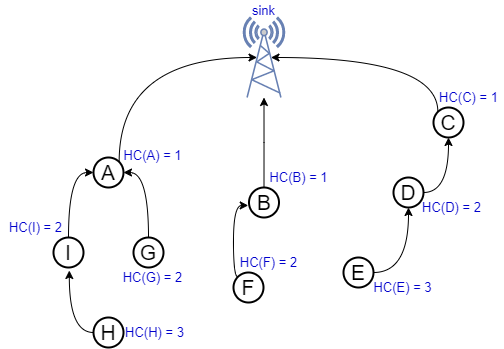
\includegraphics[width=1.1\linewidth]{Contents/Images/graphs/interestDissemination/hopCount.png}
  \end{subfigure}
  \caption{Stato della rete una volta finita la fase di Interes Dissemination}
  \label{fig:hopCount}
\end{figure}

Una volta terminata interamente la fase di \textit{Interest Dissemination}, lo stato della rete è quello mostrato in  \textbf{Figura \ref{fig:hopCount}} dove ogni nodo è a conoscenza della distanza tra se stesso e il sink. 